\documentclass{amsart}
\usepackage{graphicx}
\graphicspath{{./}}
\usepackage{hyperref}
\usepackage{csvsimple}
\usepackage{longtable}
\usepackage{epigraph}
\title{Zulf's Invariance of Pairwise Joint Distribution of Values for Bad People}
\author{Zulfikar Moinuddin Ahmed}
\date{\today}
\begin{document}
\maketitle

I report approximate invariance for joint probability distribution of reduced moral values for bad people.

By Values I refer to Q177--Q195 of World Values Survey Wave 7.

I remap the answers into classes $(1,2,3)\rightarrow Good$, then $(4,5,6,7)\rightarrow Gray$ and $(8,9,10)\rightarrow 3$.

We show that regardless of the pair of questions we pick, the pairwise joint frequency is roughly invariant.

\section{Result}

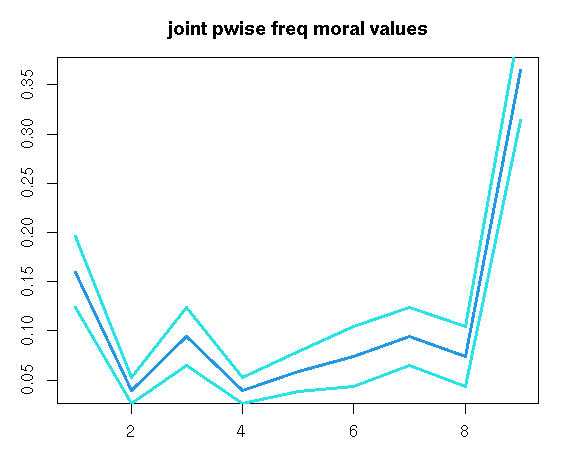
\includegraphics[scale=0.8]{jpwfreq.jpeg}

In the graph above, you can see the 1-standard deviation from the mean frequency of the $3\times 3$ table for all pairs of variables.  

\section{Method to Invariance}

We collapse 1-10 to 1,2,3 representing Good, Gray,Bad.  Then we compute the actual joint probability distribution, a $3\times 3$ matrix.    Noise is relatively small enough to conclude invariance.

This result is an extremely non-trivial result.  There is no reason that occurred to me  for why joint pairwise frequencies ought to be invariant at all in this case.  My own intuition about human moral nature is based on expecting -- wrongly it turns out -- character to fix the class in Good, Gray, Bad for many of the survey questions.  Instead, there is some {\em regular stochasticity} and that is highly nontrivial and a purely empirical discovery.  Stochasticity in moral Nature of individuals was not even part of the discussion in moral philosophy or psychology in any part of Western or Eastern intellectual history.  That is purely my empirical discovery.  And here we have highly nontrivial regularity that cannot be discussed in the language of morality that has existed in West or East at all.  Regularity in frequency for Markov chains do have a lot of interesting consequences but these have never actually been considered relevant for understanding Moral Nature of Man at all previously.  This empirical discovery allows us to consider moral questions in this stochastic setting.

\end{document}